\chapter{Adversarial Learning}
In this lecture, we will discuss adversarial attack $\&$ defense for the neural network. 
We will give mathematical descriptions about attack and defense, and discuss the current trend in this field. 
\section{Introduction to Adversarial Learning}
\paragraph{Motivation}
The earliest research on the adversarial attack is on \citep{43405} and \citep{42503}, where \citep{42503} shows that a small but specified designed perturbation of image changes the prediction of a neural net,
while \citep{43405} presents an example that a panda image with a small perturbation still looks like the same for humans, but it is classified as a gibbon by the neural network.
\begin{figure}[H]
\centering
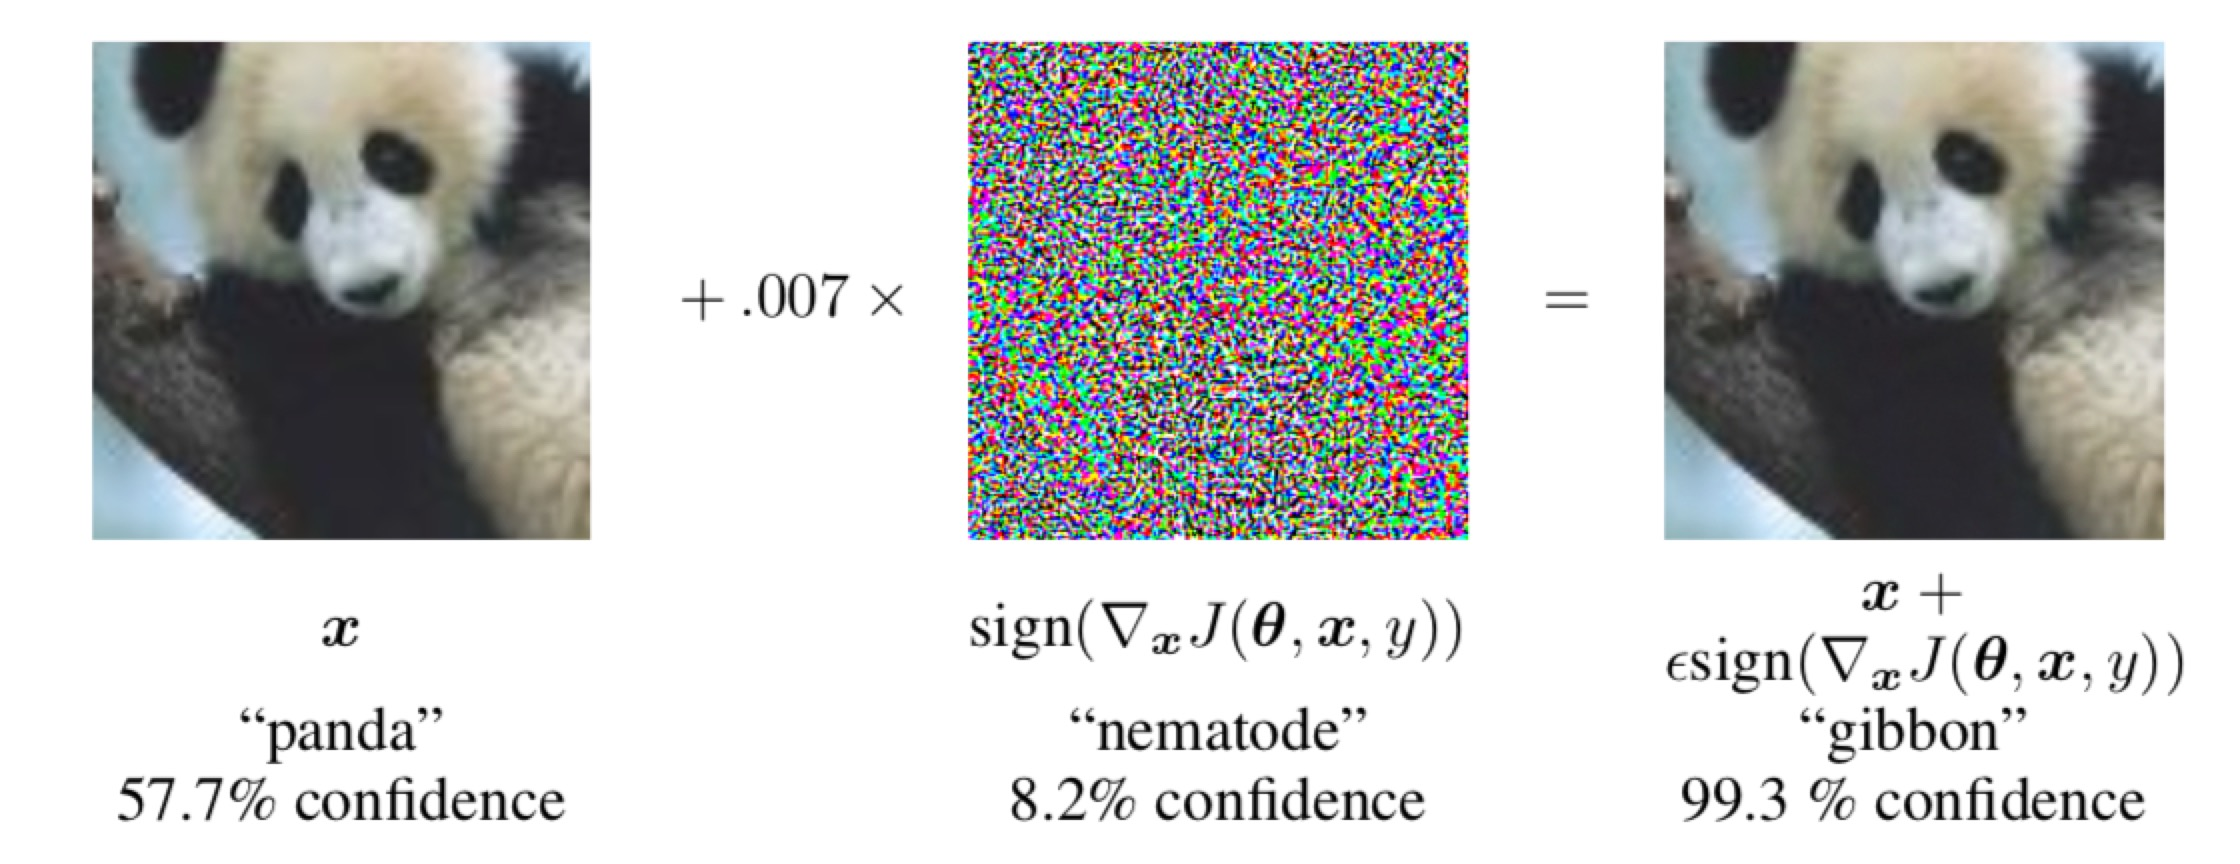
\includegraphics[width=0.7\textwidth]{Eigth_lecture/f_2}
\end{figure}
\begin{remark}
Some comments on this adversary example:
\begin{enumerate}
\item
An adversary attack is usually performed on several well-known deep learning models, such as \emph{GooLeNet}.
\item
The performance of an adversary attack is the \emph{Robust Error}, i.e., the proportion of data samples that can be effectively attacked by our attacking method.
In \citep{43405}, the robust error was $87.5\%$ on the CIFAR-10 dataset, which was later increased to $100\%$ by the $C\& W$ attack in \citep{7958570}.
Therefore, each image can be easily attacked.
\item
Transferability issue: adversarial examples designed for one kind of neural-nets can attack other kinds of neural-nets.
\item
The targetted attack is also easy, i.e., we can manipulate the prediction to whatever target we want.
\item
It is hard to defend.
\item
A good attack can achieve
\begin{itemize}
\item
high robust error;
\item
small number of queries of the model;
\item
low magnitude of perturbation.
\end{itemize}
\end{enumerate}
\end{remark}

\paragraph{Type of attacks}
Based on whether the hacker knows the model or not,
adversarial attacks can be classified as:
\begin{itemize}
\item
White box attack: the hacker can access everything of the victim model;
\item
Black box attack: the hacker can only access top-$k$ confidence scores or labels.
\end{itemize}
Based on whether the attack is aimed to manipulate the prediction, adversarial attacks can be classified as:
\begin{itemize}
\item
Targetted attack: an example in class-A is classified into class-B;
\item
Untargeted attack: an example in class-A is classified into a class other than A.
\end{itemize}
Based on what kinds of data the hacker can access, 
adversarial attacks can be classified as:
\begin{itemize}
\item
Evasion attack: the hacker can change  testing data.
We focus on this kind of attack in this lecture
\item
Poison attack: the hacker can change the training data.
\end{itemize}

\paragraph{Bibliography}
In 2014, the papers \citep{43405} and \citep{42503} were the first ones that introduced white-box attacks;
In 2016, the papers \citep{7958570} introduced black-box attacks;
In 2017, \citep{Chen2017} first performed the black box attacks by zeroth-order optimization methods;
In 2018, \citep{Ilyas2018} introduced the zeroth-order attacks by querying the objective as less as possible.

\section{Mathematical Formulation of Adversary Attack}
Consider the supervised setting, i.e., given the data points $\{(x_i,y_i)\}_{i=1}^n$, the modeler wants to generate a neural network $f_{\theta}$ such that $f(\theta;x_i)\approx y_i$ for each $i$.
Now we give various formulations for different types of attacks.

\subsection{Un-targetted Attack}
The goal of an untargeted attacker is that given a data instance $x$, the perturbed input $x+\delta$ will make the neural-nets learn a wrong model.
This gives an optimization formulation:
\begin{subequations}\label{Eq:8:1}
\begin{align}
\min_{\delta\in\mathbb{R}^d}\qquad&\|\delta\|_p\label{Eq:8:1:a}\\
\text{s.t.}\qquad&f(x+\delta)\ne y\label{Eq:8:1:b}\\
&x+\delta \in[0,1]^d\label{Eq:8:1:c}
\end{align}
where (\ref{Eq:8:1:a}) is to make the energy of the pertubation as small as possible;
(\ref{Eq:8:1:b}) is to mislead the model;
(\ref{Eq:8:1:c}) is to make the perturbed input well-defined.
\end{subequations}
The inequality constraint~(\ref{Eq:8:1:b}) makes the problem hard to solve. Thus we often reformulates this problem as
\begin{subequations}
\begin{align}
\max\qquad&J(f(x+\delta),y)\label{Eq:8:2:a}\\
\text{s.t.}\qquad&\|\delta\|_p\le\epsilon\label{Eq:8:2:b}\\
&x+\delta \in[0,1]^d
\end{align}
where $J(\cdot,\cdot)$ is some loss function;
the objective (\ref{Eq:8:2:a}) is to 
maximize the loss between output for perturbed data and original one;
the constraint (\ref{Eq:8:2:b}) is to keep the perturbation in a small magnitude $\varepsilon$.
The decision variable in this problem is the input perturbation $\delta$ instead of parameters in the neural-nets $f$.
\end{subequations}

The \emph{fast gradient sign method}~(FGSM)~\citep{43405} can be used to solve this optimization problem.
First linearize the objective (\ref{Eq:8:2:a}) and project it into the norm constrained set, 
we imply that the update should be 
\[
\eta=\epsilon\cdot\text{sign}(\nabla_xJ(f(x),y)),
\]
and the adversarial attack is performed by setting
$\tilde{x} = x + \eta$. 
\begin{figure}[H]
\centering
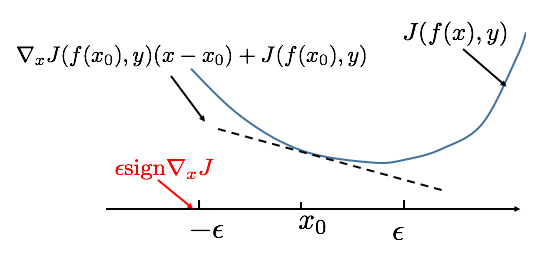
\includegraphics[width=\textwidth]{Eigth_lecture/f_3}
\caption{Illustration for Fast gradient sign method}
\end{figure}
The update rule is very easy, and only one-time update is performed.
\subsection{Targetted Attack}
The goal of targetted attack is to add a perturbation such that the output label is a specific class.
Suppose that the target class is $t\in\{1,\dots,M\}$. Similar to the idea in un-targetted attack, the typical formulation is 
\begin{subequations}\label{Eq:8:3}
\begin{align}
\min_{\delta\in\mathbb{R}^d}\qquad&\|\delta\|_p\label{Eq:8:3:a}\\
\text{s.t.}\qquad&f(x+\delta)=t\label{Eq:8:3:b}\\
&x+\delta \in[0,1]^d\label{Eq:8:3:c}
\end{align}
\end{subequations}
This kind of attack is called \emph{Carlini-Wagner} attack, proposed in the paper \citep{7958570}.
Solving (\ref{Eq:8:3}) is in general harder than solving (\ref{Eq:8:1}).
We view this problem as an equality-constrained optimization, which can be solved using \emph{penalty method}:
\begin{itemize}
\item
Step 1: Find a function $g(\cdot)$ such that 
\[
g(\tilde{x})\le0\implies f(\tilde{x})=t
\]
\begin{itemize}
\item
For example, construct $g(\tilde(x)) = \bigg(\frac{1}{2} - [Z(\tilde{x})]_t\bigg)_+$, whre $([Z(\tilde{x})]_{t})_{t=1}^M$ is the output before the softmax layer.
If $g(\tilde(x))\le0$, then the $t$-th entry before the softmax layer is larger than $\frac{1}{2}$, i.e., $f(\tilde{x})=t$.
\item
Similar to the idea above, construct
\[
g(\tilde{x})=\bigg(\max_{i\ne t}\{[Z(\tilde{x})]_i\} - [Z(\tilde{x})]_t\bigg)_+
\]

\end{itemize}
\item
Step 2: Penalize the equality constraint into the objective function:
\begin{subequations}\label{Eq:8:4}
\begin{align}
\min_{\delta}\qquad&\|\delta\|_p + c\cdot g(x+\delta)\\
\text{s.t.}\qquad&x+\delta \in[0,1]^d
\end{align}
\end{subequations}
\end{itemize}


\paragraph{Solving Optimization Problems in Adversary Attack}
Either Zeroth-order or First-order optimization algorithm can be used to solve the problems like (\ref{Eq:8:1}) or (\ref{Eq:8:4}). 
The advantage of first-order methods, such as projected gradient descent and Adam~\citep{kingma-adam}, are fast convergence rates, but they need the gradient information, i.e., using backpropagation of the neural-nets, i.e., white box attack is needed, which is in-practical in life. 
Therefore, people consider the zeroth-order methods, also called the \emph{derivative-free methods}.
This method estimates gradient information using objective evaluation. However, this method is \emph{slower} than gradient methods, by order of low polynomial of problem dimension.

\subsection{Zeroth-order Optmization}
The basic ideas of zeroth-order methods are to approximate the gradient information by calling objective value several times.
At point $x$, the Gausaain vector $u$ is generated with correlation $B^{-1}$.
Then the gradient at $x$ can be approximated as:
\[
g_\mu(x) = \frac{f(x+\mu u) - f(x)}{\mu} \cdot Bu,
\]
or
\[
\hat{g}_\mu(x) = \frac{f(x+\mu u) - f(x-\mu u)}{2\mu}\cdot Bu.
\]
Given $T$ iterations for running the algorithm, the optimality measures are $h_T:=\mathbb{E}[f(x_T)] - f^*$ for convex problems, or $\tilde{h}_T:=\mathbb{E}[\|\nabla f(x_T)\|^2]$ for non-convex problems.
The typical zeroth order method is the random gradient free algorithm~\citep{Nesterov2011}, i.e., in each iteration perform the gradient-descent-like update:
\[
x_{k+1} = x_k - hB^{-1}g_\mu(x_k).
\]
For convex objective $f$, $h_T=\mathcal{O}(d/T) + \mathcal{O}(\epsilon)$, where $d$ is the problem dimension. To achieve $h_T\le\epsilon$, $T=\mathcal{O}(d/\epsilon)$ iterations are needed.
For non-conex $f$, $\tilde{h}_T=\mathcal{O}(d/T) + \mathcal{O}(\epsilon)$.
To achieve $\tilde{h}_T\le\epsilon$, $T=\mathcal{O}(d/\epsilon)$ iterations are needed.


\section{Adversarial Defense}
Currently, there are two kinds of defense strategies:
\begin{itemize}
\item
Adversarial training: Defender generates training data using a known attack, and then tries to improve his model. 
However, the model may still be vulnerable under new kinds of attacks. 
Moreover, it does not perform very well even for given attacks.
\item
Defensive distilling: 
Based on distilling the network knowledge, which is effective, i.e.,  reducing robust error from $95\%$ to $5\%$. However, it does not perform well for the $C\& W$ attacks
\end{itemize}
\subsection{Certified Defense}
This defense method borrows the idea of robust optimization, which aims to solve the min-max problem:
\begin{subequations}
\begin{align}
\min_{\theta}\mathbb{E}_{(x,y)\sim\mathbb{P}}\qquad&\max_{\tilde{x}}\left[1\{f_\theta(\tilde{x})\ne y\}\right]\label{Eq:8:5:a}\\
\text{s.t.}\qquad&\|\tilde{x} - x\|_p\le\varepsilon\label{Eq:8:5:b}
\end{align}
\end{subequations}
The objective (\ref{Eq:8:5:a}) is to minimize the percentage of getting an error among all samples, and the constraint (\ref{Eq:8:5:b}) assumes the perturbation magnitude is bounded by $\varepsilon$.

The state of art for certified defense method is shown in the following table~\citep{SPA3327757}:
\begin{center}
\begin{table}[H]
\centering
\begin{tabular}{|l|l|l|}
\hline
Accuracy 				   & MINST & CIFAR-10   \\
 $\varepsilon=0.1$   & $3\%$   &     $34\%$  \\
 $\varepsilon=0.3$   & $34\%$   &      \\
 $\varepsilon=2/255$   &  &     $36\%$  \\
  $\varepsilon=2/255$   &  &     $70\%$  \\
  \hline
\end{tabular}
\caption{The entries in the table are the robust error,
the $\varepsilon$ denotes the norm of perturbation.
}
\end{table}
\end{center}
Generally speaking, it is very challenging to make models robust to different kinds of attacks. 
It is still an active research area.

\section{Optimization Algorithms}

\subsection{Part I: Gradient Descent~(GD) method}
Consider the unconstrained problem
\[
\min_{x}f(x)
\]
Apply the Gradient Descent~(GD) method:
\[
x^{k+1} = x^k - \gamma\nabla f(x^k)
\]
Following questions need to be considered:
\begin{enumerate}
\item
When does the algorithm work?
\begin{itemize}
\item
Assumption for the problem:
\begin{enumerate}
\item
The objective function is $L$-smooth;
\item
The level set $X_{\delta}=\{x\mid f(x)\le \delta\}$ is bounded for all $\delta$.
\end{enumerate}
\end{itemize}
\item
What kind of solution can it compute?
\begin{itemize}
\item
It finds the $\epsilon$-first-order-stationary-points, i.e., $x$ such that $\|\nabla f(x)\|\le\epsilon$.
\end{itemize}
\item
How fast can we compute it?
\begin{itemize}
\item
Sublinear convergence rate.
We encourage the reader to first go through the convergence proof for convex objective functions in the appendix. The related contents are typed on the undergraduate course MAT3220, \emph{Optimization II}.
\end{itemize}
\end{enumerate}

By assuming that $f$ is $L$-lipschitz which is not necessarily convex, we give a convergence proof for the gradient descent method.
\begin{theorem}
Suppose that the objective function $f$ is $L$-lipschitz, and gradient descent method is applied in each iteration:
\[
x^{k+1} = x^k-\frac{1}{L}\nabla f(x^k).
\]
Define $T^*:=\min\{i: \|\nabla f(x^i)\|^2\le\epsilon\}$, then $T^*=\mathcal{O}(1/\epsilon)$. 
\end{theorem}


\begin{proof}
\begin{enumerate}
\item
Step 1: GD method always makes significant progress in each iteration.
\begin{subequations}
\begin{align}
f(x^{r+1})-f(x^r)&\le  \inp{\nabla f(x^r)}{x^{r+1} - x^r} + \frac{L}{2}\|x^{r+1}-x^r\|^2\label{Eq:8:6:a}\\
&\le -\frac{1}{L}\|\nabla f(x^r)\|^2+\frac{L}{2}\|x^{r+1}-x^r\|^2\label{Eq:8:6:b}\\
&\le -\frac{1}{2L}\|\nabla f(x^r)\|^2\label{Eq:8:6:c}
\end{align}
where (\ref{Eq:8:6:a}) is by the Lipschitzness of $f$;
(\ref{Eq:8:6:b}) is by the identity $x^{r+1} - x^r=-1/L\nabla f(x^r)$;
(\ref{Eq:8:6:c}) is by the inequality $\|x^{r+1}-x^r\|\le\frac{1}{L}\|\nabla f(x^r)\|$.
\end{subequations}
\item
Step 2: Considering the best performance in first $T^*$ iteration.

By (\ref{Eq:8:6:c}), we imply
\begin{equation}
f(x^\infty)-f(x^0)\le -\frac{1}{2L}\sum_{r=0}^\infty\|\nabla f(x^r)\|^2
\end{equation}
Moreover, since $T^*$ is the first iteration where the iterate reaches the $\epsilon$-suboptimality point,
\begin{align*}
\epsilon&\le \frac{1}{T^*}\sum_{r=1}^{T^*}\|\nabla f(x^r)\|^2\\
&\le \frac{1}{T^*}\sum_{r=0}^\infty\|\nabla f(x^r)\|^2\le \frac{2L}{T^*}[f(x^0) - f(x^\infty)]
\end{align*}
It follows that
\[
T^*\le \frac{2L[f(x^0) - f(x^\infty)]}{\epsilon}=\mathcal{O}(1/\epsilon).
\]
\end{enumerate}
\end{proof}





\begin{remark}
\begin{enumerate}
\item
The convergence order does matter, but before caring about that, we need to pay attention to the \emph{optimality measure}, i.e., whether $\|\nabla f(x)\|\le\epsilon$ or $\|\nabla f(x)\|^2\le\epsilon^2$.
\item
To reach $\epsilon$-FOSP, we need $\mathcal{O}(1/\epsilon^2)$ iteration;
in deep learning training, the gradient descent operation in each iteration is expansive.
\item
The gradient descent, if converge, then it converges to SOSP with probability one, and it will 
escape strict saddle points.

However, the gradient descent does not necessarily converge to SOSP. 
Moreover, the convergence of gradient descent to SOSP is too slow, and perturbation can rescue this situation.
Take one special optimization as an example.
\begin{figure}[H]
\centering
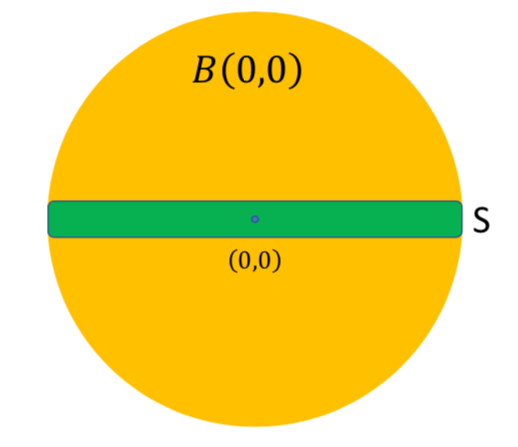
\includegraphics[width=0.6\textwidth]{Eigth_lecture/f_4}
\caption{Gradient Descent cannot escape saddle point efficiently}
\end{figure}
The objective is a quadratic function
\[
f(x)=\frac{1}{2}x\trans\begin{pmatrix}
1&0\\0&-1
\end{pmatrix}x
\]
The gradient descent formula is given by:
\[
x^{k+1}=\begin{pmatrix}
1-\gamma&0\\0&1+\gamma
\end{pmatrix}
\]
In this case, the gradient descent will get stuck around the line of the saddle point $(0,0)$,
but perturbed gradient descent motivates the iterates to explore more areas around the saddle point.
\end{enumerate}
\end{remark}

In the next lecture, modern optimization methods will be introduced.





















%Adversarial Learning:
%\begin{itemize}
%\item
%Adversarial Examples.
%\item
%Formulation ``Attack''.
%\item
%Denfense formulations.
%\item
%Current Work
%\end{itemize}
%
%Optimization Algorithms:
%\begin{itemize}
%\item
%GD, SGD, momentum methods.
%\end{itemize}



